\documentclass[compress]{beamer}
\usepackage{ifthen,verbatim}

\newcommand{\isnote}{}
\xdefinecolor{lightyellow}{rgb}{1.,1.,0.25}
\xdefinecolor{darkblue}{rgb}{0.1,0.1,0.7}

%% Uncomment this to get annotations
%% \def\notes{\addtocounter{page}{-1}
%%            \renewcommand{\isnote}{*}
%% 	   \beamertemplateshadingbackground{lightyellow}{white}
%%            \begin{frame}
%%            \frametitle{Notes for the previous page (page \insertpagenumber)}
%%            \itemize}
%% \def\endnotes{\enditemize
%% 	      \end{frame}
%%               \beamertemplateshadingbackground{white}{white}
%%               \renewcommand{\isnote}{}}

%% Uncomment this to not get annotations
\def\notes{\comment}
\def\endnotes{\endcomment}

\setbeamertemplate{navigation symbols}{}
\setbeamertemplate{headline}{\mbox{ } \hfill
\begin{minipage}{5.5 cm}
\vspace{-0.75 cm} \small
\end{minipage} \hfill
\begin{minipage}{4.5 cm}
\vspace{-0.75 cm} \small
\begin{flushright}
\ifthenelse{\equal{\insertpagenumber}{1}}{}{Jim Pivarski \hspace{0.2 cm} \insertpagenumber\isnote/\pageref{numpages}}
\end{flushright}
\end{minipage}\mbox{\hspace{0.2 cm}}\includegraphics[height=1 cm]{../cmslogo} \hspace{0.1 cm} \includegraphics[height=1 cm]{../tamulogo} \hspace{0.01 cm} \vspace{-1.05 cm}}

\begin{document}
\begin{frame}
\vfill
\begin{center}
\textcolor{darkblue}{\Large Status of CSC Beam-Halo Alignment}

\vfill
\begin{columns}
\column{0.3\linewidth}
\begin{center}
\large
\textcolor{darkblue}{Jim Pivarski}
\end{center}
\end{columns}

\begin{columns}
\column{0.3\linewidth}
\begin{center}
\scriptsize
{\it Texas A\&M University}
\end{center}
\end{columns}

\vfill
24 November, 2009

\end{center}
\end{frame}

%% \begin{notes}
%% \item This is the annotated version of my talk.
%% \item If you want the version that I am presenting, download the one
%% labeled ``slides'' on Indico (or just ignore these yellow pages).
%% \item The annotated version is provided for extra detail and a written
%% record of comments that I intend to make orally.
%% \item Yellow notes refer to the content on the {\it previous} page.
%% \item All other slides are identical for the two versions.
%% \end{notes}

\small

\begin{frame}
\frametitle{Summary}
\begin{itemize}
\item We have beam-halo data!  But at the end of the chain, not many events (about 150)
\begin{itemize}
\item this might have been clarified in Andy, Gian Piero, and Jinzhong's talk
\item I haven't found any leaks in the offline pipeline
\end{itemize}

\item No alignment yet, but we can see that the raw
  distributions agree well with intuition and expectations from Monte Carlo

\item New features in the algorithm
\begin{itemize}\setlength{\itemsep}{0.1 cm}
\item if a CSC chamber or CLCT 1 or 5 is missing, breaking the ring, we can
  now use the closure ($\sum \mbox{residuals} = 0$) as a constraint to perform an alignment

\item ME1/1a and ME1/1b are now treated as rigidly-connected

\item additional anti-cosmic and beam-splash cuts

\item lots of new plots to keep an eye on things (especially the cuts)
\end{itemize}

\item Thorough Monte Carlo tests with the same parameters as data
\end{itemize}
\end{frame}

\begin{frame}
\frametitle{Event counts}

\vspace{0.5 cm}
\hfill \includegraphics[height=2.5 cm]{overlaps.png}

\vspace{-3 cm}
\begin{itemize}
\item Reminder: we're looking for tracks that pass through \\ the overlap region of pairs of CSC chambers--- \\ about 7\% of the total beam-halo rate because of \\ geometric acceptance

\item MuAlBeamHaloOverlaps (dedicated alignment sample): \\ about 170 events (as of yesterday)
\begin{itemize}
\item prompt reco: includes data up to 122281 {\scriptsize (Monday 9:30 GMT)}
\item trigger configuration:
\begin{itemize}
\item HLT\_CSCBeamHalo* only until Monday morning
\item all muon triggers {\scriptsize (including HLT\_L1OpenMuon*)} thereafter
\end{itemize}
\item almost all events are in three runs only:
\begin{itemize}
\item 121964, 20 Nov 21:30, 72 events
\item 122269, 23 Nov  4:50, 61 events
\item 122270, 32 Nov  5:20, 35 events
\end{itemize}
\end{itemize}

\item ExpressMuon/ExpressPhysics: the MuAlBeamHaloOverlaps selection algorithm {\scriptsize (without HLT requirement)} returns 20 events because most of them have zero ``cosmicMuon'' tracks

\item ZeroBias: selection returns 1380, but nearly all are cosmic rays
\end{itemize}
\end{frame}

\begin{frame}
\frametitle{Occupancy distributions}

\begin{columns}
\column{0.7\linewidth}
\includegraphics[width=\linewidth]{REAL_occupancy1.pdf}

\includegraphics[width=\linewidth]{MCBeamHalo_occupancy1.pdf}

\column{0.35\linewidth}
\begin{itemize}
\item Tracks crossing {\it pairs} of chambers (multiply by 2 for total segments)

\item Top: data \\ Bottom: MC

\item Only low-rate ring-2 collected because ring-1 was at low voltage {\scriptsize (STANDBY)} for safety

\item MC $\phi$ and $R$ distributions are not \mbox{realistically simulated\hspace{-1 cm}} \\ {\scriptsize (ATLAS cavern)}

\end{itemize}
\end{columns}
\end{frame}

\begin{frame}
\frametitle{For comparision: CSCValidation}

\begin{itemize}
\item CSCValidation segment occupancy plots for the three runs
\item Confirms higher rate in ring-2
\end{itemize}

\vfill
\includegraphics[width=0.5\linewidth]{CSCValidation_segments_121964.png} \fbox{\includegraphics[width=0.6\linewidth]{REAL_occupancy1.pdf}}

\includegraphics[width=0.5\linewidth]{CSCValidation_segments_122269.png} \includegraphics[width=0.5\linewidth]{CSCValidation_segments_122270.png}
\end{frame}

\begin{frame}
\frametitle{Hit distributions (MC)}

\begin{columns}
\column{0.7\linewidth}
\includegraphics[width=\linewidth]{MCBeamHalo_positions1.png}

\includegraphics[width=\linewidth]{MCBeamHalo_positions2.png}

\column{0.35\linewidth}
\begin{itemize}
\item Top: $Y$ vs.\ $X$ \\ Bottom: $R$ vs.\ $\phi$

\item Both are MC

\item Radial spokes along CSC edges indicate that overlap selection works

\item ME1 $R < 140$~cm missing due to beam-halo
  trigger requirements (highlighted in yellow)

\item ME1/1a chambers must be glued to ME1/1b or they'll be lost!
\end{itemize}
\end{columns}
\end{frame}

\begin{frame}
\frametitle{Event display pictures (data)}

\begin{itemize}
\item $\sim$90 beam-halo/gas, $\sim$10 beam-splashes, and $\sim$70 cosmics
\item Zooming into a nice beam-halo event:
\end{itemize}

\begin{center}
\includegraphics[width=0.33\linewidth]{overlap_closeup04.png} \hspace{0.05 cm}
\includegraphics[width=0.33\linewidth]{overlap_closeup03.png}

\vspace{0.1 cm}
\includegraphics[width=0.33\linewidth]{overlap_closeup02.png} \hspace{0.05 cm}
\includegraphics[width=0.33\linewidth]{overlap_closeup01.png}
\end{center}
\end{frame}

\begin{frame}
\frametitle{Offline cuts}
\label{thispage}

\begin{itemize}
\item Top plots: data, bottom plots: pure beam-halo Monte Carlo
\end{itemize}

\begin{columns}
\column{0.25\linewidth}
Anti-beam-splash: \\ \# segments $<$ 30 \\ \mbox{ }

\includegraphics[width=\linewidth]{REAL_num_segments.pdf}

\includegraphics[width=\linewidth]{MCBeamHalo_num_segments.pdf}

\column{0.25\linewidth}
Anti-cosmic: point to beamline ($\pm$2.5~mrad)

\includegraphics[width=\linewidth]{REAL_beamline_pointing.pdf}

\includegraphics[width=\linewidth]{MCBeamHalo_beamline_pointing.pdf}

\column{0.25\linewidth}
Exclude last cathode strip: hit error $<$ 2~mm

\includegraphics[width=\linewidth]{REAL_hit_error.pdf}

\includegraphics[width=\linewidth]{MCBeamHalo_hit_error.pdf}

\column{0.25\linewidth}
Fiducial segments: \\ \mbox{\#hits/segment $\ge$ 4\hspace{-1 cm}} \\ (usually require 6)

\includegraphics[width=\linewidth]{REAL_hits_on_segments.pdf}

\includegraphics[width=\linewidth]{MCBeamHalo_hits_on_segments.pdf}

\end{columns}
\end{frame}

\begin{frame}
\frametitle{Residuals}

\begin{columns}
\column{0.7\linewidth}
\includegraphics[width=\linewidth]{REAL_residuals.pdf}

\includegraphics[width=\linewidth]{MCBeamHalo_residuals.pdf}

\column{0.4\linewidth}

\begin{itemize}
\item Top: data, bottom: MC

\item $\Delta (r\phi)$ and $\Delta \frac{d(r\phi)}{dz}$:
\end{itemize}

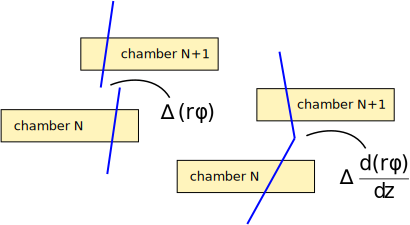
\includegraphics[width=\linewidth]{residuals_diagrams.pdf}

\begin{itemize}
\item Error in $\Delta (r\phi)$ dominated by $\Delta \frac{d(r\phi)}{dz}$ resolution

\item If \#hits/segment $=$ 6 (all segments must be fiducial), \mbox{MC resolutions\hspace{-1 cm}} \\ improve by 20\%
\end{itemize}
\end{columns}
\end{frame}

\begin{frame}
\frametitle{MC alignment accuracy}

\textcolor{darkblue}{All rings:}

\includegraphics[width=0.9\linewidth]{MCBeamHalo-all_align_step6.pdf}

\vspace{0.2 cm}
\textcolor{darkblue}{ME2/1, ME3/1, ME4/1}

\includegraphics[width=0.9\linewidth]{MCBeamHalo-inner_align_step6.pdf}

\begin{itemize}
\item Grain of salt needed: MC $\phi$ and $R$ distributions are unrealistic

\item Bottleneck seems to be $\phi_y$ (mean of $\Delta \frac{d(r\phi)}{dz}$ residuals), which can be determined better with tracker tracks from cosmics or collisions
\end{itemize}
\end{frame}

\begin{frame}
\frametitle{Incomplete ring alignment}

\begin{itemize}\setlength{\itemsep}{0.2 cm}
\item New feature: can now align incomplete rings by {\it assuming}
\begin{center}
$\displaystyle \sum_i^N \Delta (r\phi)_i = 0$ \hspace{0.5 cm}and\hspace{0.5 cm} $\displaystyle \sum_i^N \Delta \frac{d(r\phi)}{dz}_i = 0$
\end{center}

\item Closure test is no longer available as a cross-check for these rings

\item Only works for certain topologies:
\end{itemize}

\vfill
\includegraphics[width=\linewidth]{incomplete_rings.pdf}

\begin{itemize}
\item For example, we can align ME$+$4/2 (third case)
\end{itemize}
\end{frame}

%% \section*{First section}
%% \begin{frame}
%% \begin{center}
%% \Huge \textcolor{blue}{First section}
%% \end{center}
%% \end{frame}

\begin{frame}
\frametitle{Connecting ME1/1a and 1/1b}
\begin{itemize}\setlength{\itemsep}{0.3 cm}
\item New feature: ME1/1a chambers and their corresponding 1/1b chambers are now treated as rigidly connected physical objects

\item ME1/1a and 1/1b chambers are separate entities in the software,
  and therefore separate in the alignment framework

\item They share the same coordinate system (in ideal geometry), so
  residuals from each 1/1a and its 1/1b counterpart can be put in
  the same bin, with the resulting alignment corrections applied to both

\item This implementation behaves properly
\begin{itemize}
\item 1/1a and 1/1b do not get out of sync
\end{itemize}
\end{itemize}
\end{frame}

\begin{frame}
\frametitle{Conclusions}
\begin{itemize}\setlength{\itemsep}{0.5 cm}
\item Beam-halo overlaps sample still has too low statistics for alignment
\begin{itemize}
\item tried to find the events in ExpressMuon, ExpressPhysics, and ZeroBias, but they aren't supersets of MuAlBeamHaloOverlaps
\end{itemize}

\item The events we have make sense
\begin{itemize}\setlength{\itemsep}{0.1 cm}
\item most events in ring-2 because ring-1 not at high voltage
\item individual event displays look like the overlap events we want
\item plots differ by beam-splash and cosmic ray backgrounds
\item fewer hits per segment than MC: inefficiency due to \mbox{lower voltage?\hspace{-1 cm}}
\item residuals consistent with $\sim$1~mm misalignment relative to ideal
\end{itemize}

\item The alignment machinery will work when needed
\begin{itemize}
\item tested in MC, including the new features
\end{itemize}
\end{itemize}
\label{numpages}
\end{frame}

\begin{frame}
\frametitle{The ZeroBias sample}

\begin{itemize}
\item The ZeroBias sample is $\sim$all cosmic rays:
\item MuAlBeamHaloOverlaps and beam-halo MC shown on page~\pageref{thispage}
\end{itemize}

\vfill
\begin{columns}
\column{0.33\linewidth}
MuAlBeamHaloOverlaps

\includegraphics[width=0.9\linewidth]{REAL_beamline_pointing.pdf}

\column{0.33\linewidth}
Pure beam-halo MC

\includegraphics[width=0.9\linewidth]{MCBeamHalo_beamline_pointing.pdf}

\column{0.33\linewidth}
ZeroBias sample

\includegraphics[width=0.9\linewidth]{beamline_pointing_ZeroBias.pdf}
\end{columns}
\end{frame}

\end{document}
